\section{Introduction}

Wearable indoor navigation systems require reliable perception of navigable
directions while remaining inexpensive, privacy-preserving, and easy to
deploy~\cite{yuNaVIPComputerVisionBased2026}. Existing approaches predominantly rely on RGB cameras, depth sensors,
or LiDAR, which provide rich visual or geometric information but increase
hardware cost and raise privacy concerns. Training these systems also requires
large annotated datasets, and multi-camera platforms often assume a
fixed sensor arrangement established during calibration~\cite{kuoRedesigningSLAMArbitrary2020}.


% Wearable navigation aids for visually impaired users inherit three costly
% dependencies: identifiable high-resolution imagery, large hand-labeled
% datasets, and a fixed, calibrated camera layout. A sensor that shifts on the
% rig violates the geometric assumptions on which these pipelines rest.

Ultra-low-resolution thermal cameras eliminate many of the deployment barriers
of conventional visual sensors, but raise a fundamental question: can reliable
navigability be inferred from such limited observations? A $32\times24$
thermal array is inexpensive, consumes little power, and does not capture
identifiable appearance. However, its limited spatial resolution
removes much of the visual information used by conventional perception
algorithms, making environment understanding substantially more difficult.
The limited field of view and information content of each thermal array
motivate the use of multiple cameras to improve environmental coverage.

% Ultra-low-resolution thermal cameras offer a cheap and inherently private
% alternative, but at a steep perceptual cost. A $32\times24$ array costs on the
% order of tens of dollars, draws little power, and is too coarse to reveal
% identity. At the same time, each tile carries very little spatial detail,
% several cameras are needed for adequate coverage, and thermal labels are slow
% to collect by hand. We investigate whether directional navigability (whether
% the left, middle, and right views are walkable or obstructed) can be estimated
% from thermal tiles alone, with no manual labels and no geometric calibration
% at inference.


This paper investigates whether ultra-low-resolution multi-view thermal
sensing provides sufficient information to estimate directional
navigability. To answer this question, we use a high-resolution RGB camera
only during data collection to automatically generate supervisory labels for
synchronized thermal observations. During deployment, the system operates
exclusively on thermal imagery, requiring neither RGB input nor geometric
calibration.


% Our framework therefore confines RGB to the data-collection stage
% (Fig.~\ref{fig:pipeline}). A
% high-resolution camera on the wearable rig records frames synchronously with
% three ultra-low-resolution thermal cameras, and a pretrained detector on the
% RGB stream assigns a navigability label to each direction. At inference, only
% the thermal tiles are available, and the model outputs a three-class state per
% direction (\textit{clear}, \textit{person}, \textit{other object}).
% Supervision is transferred through discrete labels rather than aligned pixels,
% so inference requires neither geometric calibration nor a fixed camera-to-slot
% mapping.

This paper makes four contributions. First, we introduce a training framework that uses RGB supervision only during data collection to enable thermal-only directional navigability estimation without manual thermal annotation. Second, we present a systematic comparison of representative pixel-, feature-, and decision-level fusion strategies for ultra-low-resolution thermal sensing. Third, we evaluate robustness to changes in camera placement and introduce a lightweight camera-identity correction that maintains performance under camera permutations. Finally, we contribute a wearable multi-camera dataset of synchronized RGB and ultra-low-resolution thermal observations to support future research in privacy-preserving indoor navigation.


% We compare pixel-level stitching, decision-level output fusion, and
% feature-level fusion on the three thermal views, and we evaluate slot
% permutations with and without a lightweight identity classifier that re-sorts
% tiles before inference. This paper makes three contributions. First, it
% extends RGB-supervised auto-labeling, following Gao~\textit{et al.}'s
% DareDevil~\cite{gaoDeployablePrivacyPreservingThermalBased2025}, to a
% multi-camera thermal array that requires only coarse build-time homographies
% rather than pixel-accurate cross-modal calibration, with no manual thermal
% labels and no RGB at inference. Second, it presents an empirical comparison of
% the three fusion strategies at this resolution. Third, it introduces an
% identity correction that recovers oracle-level accuracy after slot shuffles.

\begin{figure*}[!t]
  \centering
  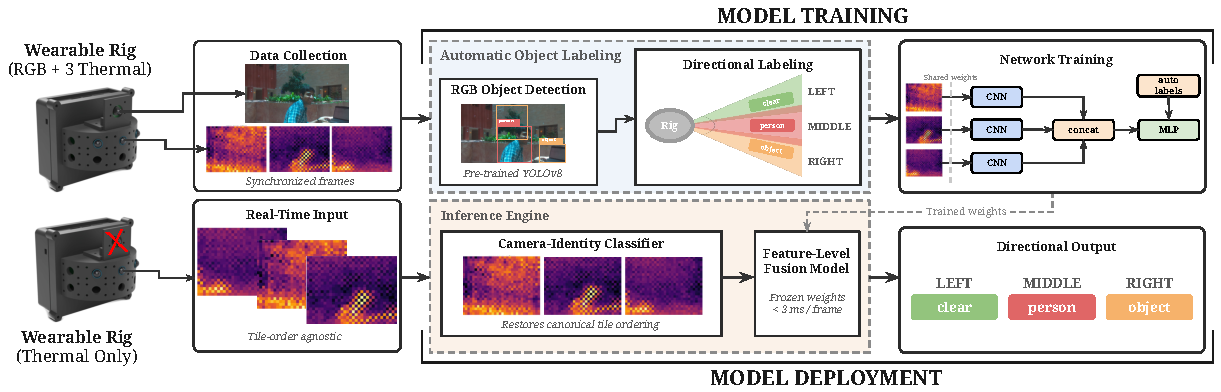
\includegraphics[width=0.9\textwidth]{figs/fig1.pdf}
  \caption{End-to-end pipeline. Top: RGB/YOLOv8 auto-labels supervise the shared-weight CNN backbone with no manual annotation. Bottom: thermal-only tiles, re-sorted by the camera-identity classifier, feed the frozen Feature Fusion model for three-class directional output. Inferno colormap for display only.}
  \label{fig:pipeline}
\end{figure*}


